\documentclass{article}

% Packages
\usepackage[english]{babel}

\usepackage[letterpaper,top=2cm,bottom=2cm,left=3cm,right=3cm,marginparwidth=1.75cm]{geometry}
\usepackage{amsmath}
\usepackage{amsfonts}
\usepackage{graphicx}
\usepackage{outlines}
\usepackage{float}
\usepackage{tabularx} % Allows for adjustable-width columns
\usepackage{graphicx} % Required for resizing table
\usepackage{booktabs} % For prettier tables
\usepackage{siunitx} % Required for alignment
\sisetup{
  table-format=-1.2,  % Specifies the format for the numbers
  table-space-text-pre = {<},  % For spacing before text
  table-space-text-post = {>},  % For spacing after text
  table-align-text-pre=false,  % Align text in the center of the space
  table-align-text-post=false,
}
\usepackage[colorlinks=true, allcolors=blue]{hyperref}

% Title
\title{Combining Expert Advice: Comparing Weighted Strategies for Enhanced Portfolio Performance}
\author{Kai Wen TAY}
\date{\today}

\begin{document}

\maketitle

\begin{abstract}
    % Abstract of your research paper
    This paper investigates the performance of different strategies for combining expert advice in the context of 13F filings from the most followed hedge funds in the United States. We thought that it would be prudent to look at what we've covered in the space of Weighted Majority Algorithms as well as the Greedy Algorithms, and see if they actually apply to a setting of stock market prediction, instead of rehashing proofs we have gone over. Specifically, we apply these algorithms to funds who have 10 years of filings for us to work with, and compare the performances of various different algorithms for combining expert advice instead of looking at how fast it converges to a expert advice. We show how a typical Weighted Majority Algorithm and a Random Weighted Majority Algorithm is able to converge to a best expert and introduce a Modified Greedy Algorithm that seems to be able to get closest in terms of performance to the best expert relative to risk and risk-reward ratio ironically.
\end{abstract}

\section{Introduction}
\label{sec:introduction}

% Introduction to your research topic
In class and in our homework in the course during the first two weeks, we covered various "No-Regret" algorithms for repeated decision making. The idea was not to combat the best adaptive strategy but just to compare ourselves with some best fixed path in hindsight. We also looked at a simple example where we thought of the idea of predicting the stock market via $n$ "expert advice". The important questions that we are trying to answer are: Is there a strategy that allows us to converge to the best expert the quickest? And does this convergence provide the best performance in terms of return and risk in terms of 13F filings from the most followed hedge funds in the United States? More importantly, if we are able to get to the best expert, does this mean that we are able to get the best performance in terms of return and risk?

I thought this topic would be interesting because this example allows us to actually quantify mistakes (i.e. how much money we earn and/or how much risk we take relative to the best expert), and provides us with some example where there is no clear way to categorise whether an expert is right or wrong (an expert in this case could have a high return but have also taken a high risk). It also gives us a chance to show how the right experts change over time and how this change actually affects the performance of different algorithms even though we converge to some expert.

We notice that if we adjust for risk and risk-reward, our algorithms can seem to converge towards weights that are similar to the best expert. We also notice that, surprisingly, in this specific case, we are able to get closest to the best expert the quickest without the need for weights or randomization. In our case of 13F filings, we see that the Modified Greedy Algorithm is able to get closest to the best expert in terms of performance.

\section{Methodology}
\label{sec:methodology}

% Description of your research methodology
This section describes the methodology we used to compare the performance of different strategies. This section will go through the data we used, how we calculated individual manager performance, risk, and return, and how we set up each of the algorithms. All of the code are available here: \url{https://github.com/derivativestester/Weighted-Majority-Experts}.

\subsection{Data}
\label{subsec:data}
All data used have been taken from WRDS database. We mainly used the 13F filings for the holdings each of the funds have quarterly, as well as CRSP data for the daily stock prices. In terms of selection, we used the top funds available on \url{https://hedgefollow.com/top-hedge-funds.php}, and took the funds that have at least 10 years of filings (this gave us 11 funds to work with). Given that CRSP data only covers stocks in the US, we only considered the long US stocks in the 13F filings. 

We then calculated the quarterly returns, standard deviation for each of the stocks in the 13F filings, and used this to calculate the individual manager performance, risk, and return (we assume each of the stocks in the 13F filings are independent for simplicity's sake).

\subsection{Algorithms Considered}
\label{subsec:algorithms}
We let $w_{i,t}$, $p_{i,t}$, $\sigma_{i,t}$ be weight, performance, and risk(standard deviation) for player $i$ as of time $t$. Then, for each expert $i$, we get cumulative value $V_{i,t}=c\prod_{t=1}^{T}(1+p_{i,t})$, where $c=$initial value of investment. Take note that in our dataframe, we have performance in the same time as weights for ease of multiplication. However, the weights are actually lagged by one time frame so we are not forward looking. We then consider the following algorithms for combining expert advice to get $\hat{V}_{t}$, $\hat{P}_{t}$, $\hat{\sigma}_{t}$, and $\hat{S}_{t}$ at time $t$ for the portfolio cumulative value, performance, risk, and risk-reward respectively:
\begin{enumerate}
    \item \textbf{Equal Weighted Strategy}: For each expert $i$, we assign a weight of $\frac{1}{n}$ such that the sum of the weights is 1, i.e.:
    $$\begin{align*}W_{t}&=\sum_{i=1}^{n}w_{i,t}=1\\
        \text{where }w_{i,t}&=\frac{1}{n}\\
        n&=\text{number of experts}\end{align*}$$
    Under this strategy, we assume that each expert is equally likely to be correct, meaning we take the average of all the experts. This gives us:
    $$\begin{align*}\hat{P}_{t}&=\sum_{i=1}^{n}w_{i,t}p_{i,t}\\
        \hat{\sigma}_{t}&=\sum_{i=1}^{n}w_{i,t}\sigma_{i,t}\\
        \hat{S}_{t}&=\frac{\hat{P}_{t}}{\hat{\sigma}_{t}}\\
        \hat{V}_{t}&=c\prod_{t=1}^{T}(1+\hat{P}_{t})\end{align*}$$
    \item \textbf{Best Experts Strategy}: For each expert $i$, we assign a weight of 1 if the expert is the Best Expert, $J$, where we define the Best Expert as:
        $$\begin{align*}\text{Condition}&=\{\text{Performance}, \text{Risk}, \text{Risk-Reward}\}\\
        J&=\begin{cases}\arg \max_{i}V_{i,T}&\text{if Condition=Performance}\\
        \arg\max_{i}-\sum_{t=1}^{T}\sigma_{i,t}&\text{if Condition=Risk}\\
        \arg\max_{i}\frac{\sum_{t=1}^{T}p_{i,t}}{\sum_{t=1}^{T}\sigma_{i,t}}&\text{if Condition=Risk-Reward}\end{cases}\end{align*}$$
    In words, we choose the expert that has the highest cumulative value, the lowest mean risk, or the highest mean risk-reward ratio. This gives us:
    $$\begin{align*}\hat{P}_{t}&=p_{J,t}\\
        \hat{\sigma}_{t}&=\sigma_{J,t}\\
        \hat{S}_{t}&=\frac{\hat{P}_{t}}{\hat{\sigma}_{t}}\\
        \hat{V}_{t}&=c\prod_{t=1}^{T}(1+\hat{P}_{t})\end{align*}$$
    This will be used as our comparison for the other algorithms.
    \item \textbf{Weighted Majority Algorithm}: In this case, we define Condition the same way we defined it for Best Experts Strategy. We also assign some arbitrary $\beta\in(0,1)$. Then, for each time $t$, we define the best expert as: $$J_{t}=\begin{cases}\arg\max_{i}p_{i,t}&\text{if Condition = Performance}\\
        \arg\max_{i}-\sigma_{i,t}&\text{if Condition = Risk}\\
        \arg\max_{i}\frac{p_{i,t}}{\sigma_{i,t}}&\text{if Condition = Risk-Reward}\end{cases}$$
    We then update the weights as follows for all time from $t=0$ to $T-1$:
    $$\begin{align*}w_{i,0}&=\frac{1}{n}\\
        w_{i,t+1}&=w_{i,t}\beta^{\text{sign}(|i-J_{t}|)}\\
        W_{t+1}&=\sum_{i=1}^{n}w_{i,t+1}\end{align*}$$
    Normalising this to sum to 1, we get:
    $$\begin{align*}\pi_{i,t}&=\frac{w_{i,t}}{W_{t}}\\
        \hat{P}_{t}&=\sum_{i=1}^{n}\pi_{i,t-1}p_{i,t}\\
        \hat{\sigma}_{t}&=\sum_{i=1}^{n}\pi_{i,t-1}\sigma_{i,t}\\
        \hat{S}_{t}&=\frac{\hat{P}_{t}}{\hat{\sigma}_{t}}\\
        \hat{V}_{t}&=c\prod_{t=1}^{T}(1+\hat{P}_{t})\end{align*}$$
    Here, in terms of optimization, we can set $$\beta=\begin{cases}\arg\max_{\beta}\hat{V}_{T}&\text{if Condition=Performance}\\
        \arg\max_{\beta}-\sum_{t=1}^{T}\hat{\sigma}_{t}&\text{if Condition=Risk}\\
        \arg\max_{\beta}\frac{\sum_{t=1}^{T}\hat{P}_{t}}{\sum_{t=1}^{T}\hat{\sigma}_{t}}&\text{if Condition=Risk-Reward}\end{cases}$$
    This is the best case scenario $\beta$ for each of the conditions but is also assuming we are prescient.
    \item \textbf{Random Weighted Majority Algorithm}: This is the same as the Weighted Majority Algorithm, but we select only one expert at random uniformly to invest in at each time $t$, i.e.:
    \begin{enumerate}
        \item First, we apply all the conditions in the Weighted Majority Algorithm to get $J_{t}$ and update the weights to get $\pi_{i,t}$ for each expert $i$.
        \item Then, we randomly select an expert $\gamma_{t}$ to invest in, i.e.:
        $$\gamma_{t} \sim \text{Categorical}(\pi_{1,t}, \pi_{2,t}, \ldots, \pi_{n,t})$$
        \item Using the selection of $\gamma_{t-1}$ for each time from $t=1$ to $T$ (note that we set equal weights at $t=0$ since we are looking backwards), we get:
        $$\begin{align*}\hat{P}_{t}&=p_{\gamma_{t-1},t}\\
            \hat{\sigma}_{t}&=\sigma_{\gamma_{t-1},t}\\
            \hat{S}_{t}&=\frac{\hat{P}_{t}}{\hat{\sigma}_{t}}\\
            \hat{V}_{t}&=c\prod_{t=1}^{T}(1+\hat{P}_{t})\end{align*}$$
    \end{enumerate}
    \item \textbf{Modified Greedy Algorithm}: We set weights in the same way as the Weighted Majority Algorithm, but we select the best expert at each time $t$ to invest in by looking at who has the highest weight at time $t-1$, i.e.:
    $$\gamma_{t}=\arg\max_{i}\pi_{i,t-1}$$
    This gives us:
    $$\begin{align*}\hat{P}_{t}&=p_{\gamma_{t},t}\\
        \hat{\sigma}_{t}&=\sigma_{\gamma_{t},t}\\
        \hat{S}_{t}&=\frac{\hat{P}_{t}}{\hat{\sigma}_{t}}\\
        \hat{V}_{t}&=c\prod_{t=1}^{T}(1+\hat{P}_{t})\end{align*}$$
\end{enumerate}

\section{Results and Analysis}
\label{sec:results-analysis}
For all our following analyses, we set initial value, $c=1000$. First, looking at all the cumulative returns for all the funds, we see that in terms of raw performance, the fund to beat is Fund 2 or 6.
%\ image of the best expert
\begin{figure}[H]
    \centering
    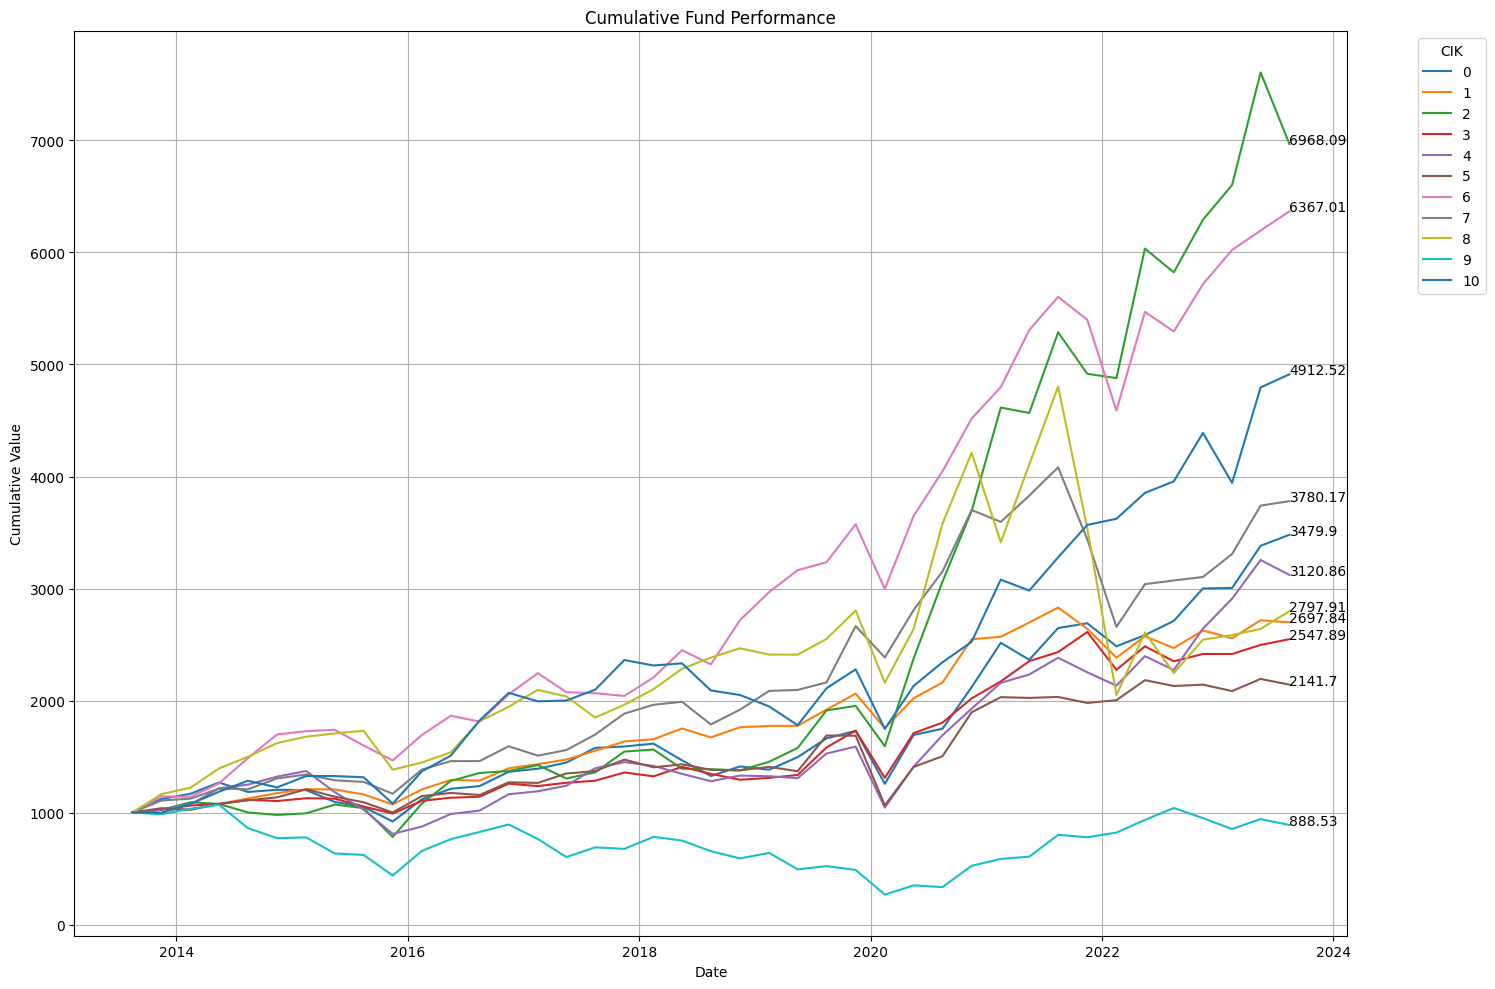
\includegraphics[width=0.9\textwidth]{cumulative_returns.png}
    \caption{Cumulative Returns for all the funds}
    \label{fig:cumulative_returns}
\end{figure}

\subsection{Equal Weighted Strategy}
\label{subsec:equal-weighted}
Looking at the equal weighted performance, we get the following results:
\begin{figure}[H]
    \centering
    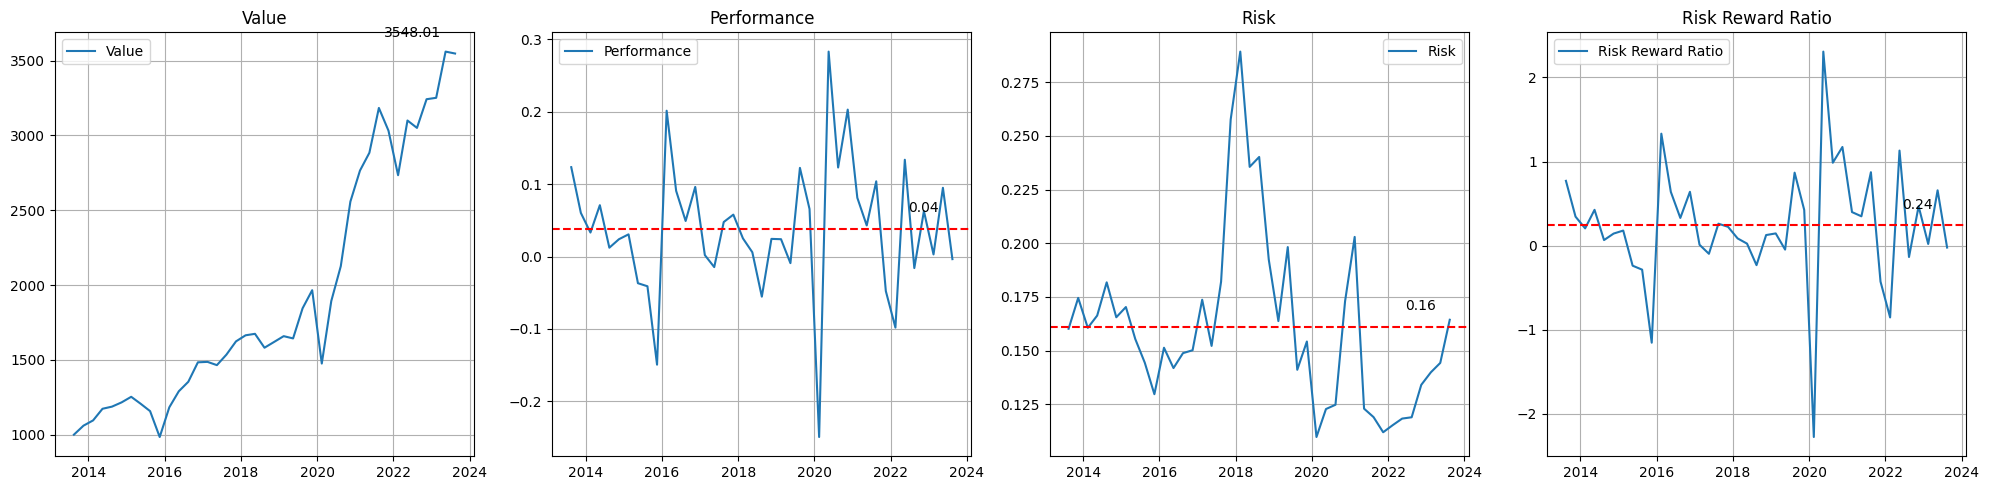
\includegraphics[width=1\textwidth]{equal_weight.png}
    \caption{Equal Weighted Strategy Performance}
    \label{fig:equal_weighted}
\end{figure}
We see that an equal weighted portfolio achieves a final value of $\$3548.01$, a mean return of $3.85\%$ quarterly. The mean risk is $16.10\%$ using a quarterly timescale, and the mean risk-reward ratio is $23.89\%$.

\subsection{Best Experts Strategy}
\label{subsec:best-experts}
Looking at the best experts strategy, we get the following results for the best expert in the space of performance, risk, and risk-reward respectively:
\begin{figure}[H]
    \centering
    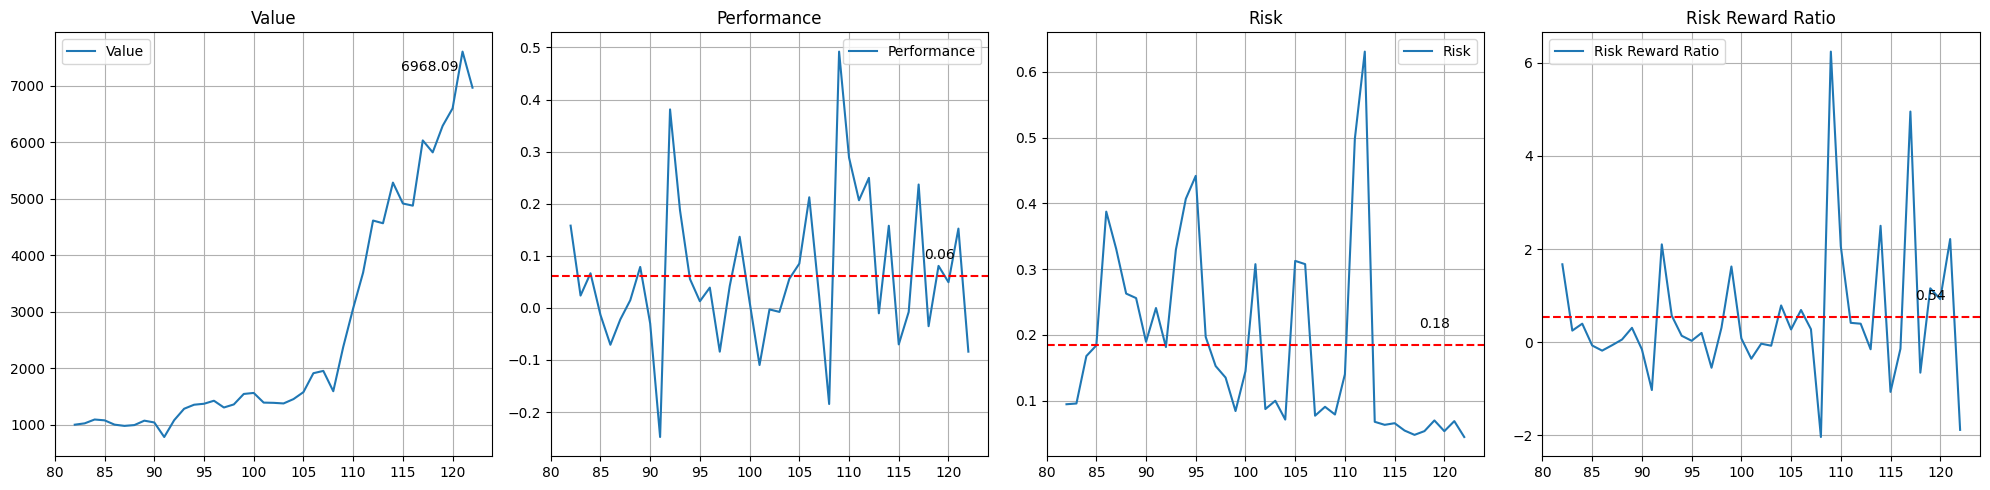
\includegraphics[width=1\textwidth]{best_experts.png}
    \caption{Best Experts Strategy Performance: Fund 2}
    \label{fig:best_experts}
\end{figure}
\begin{figure}[H]
    \centering
    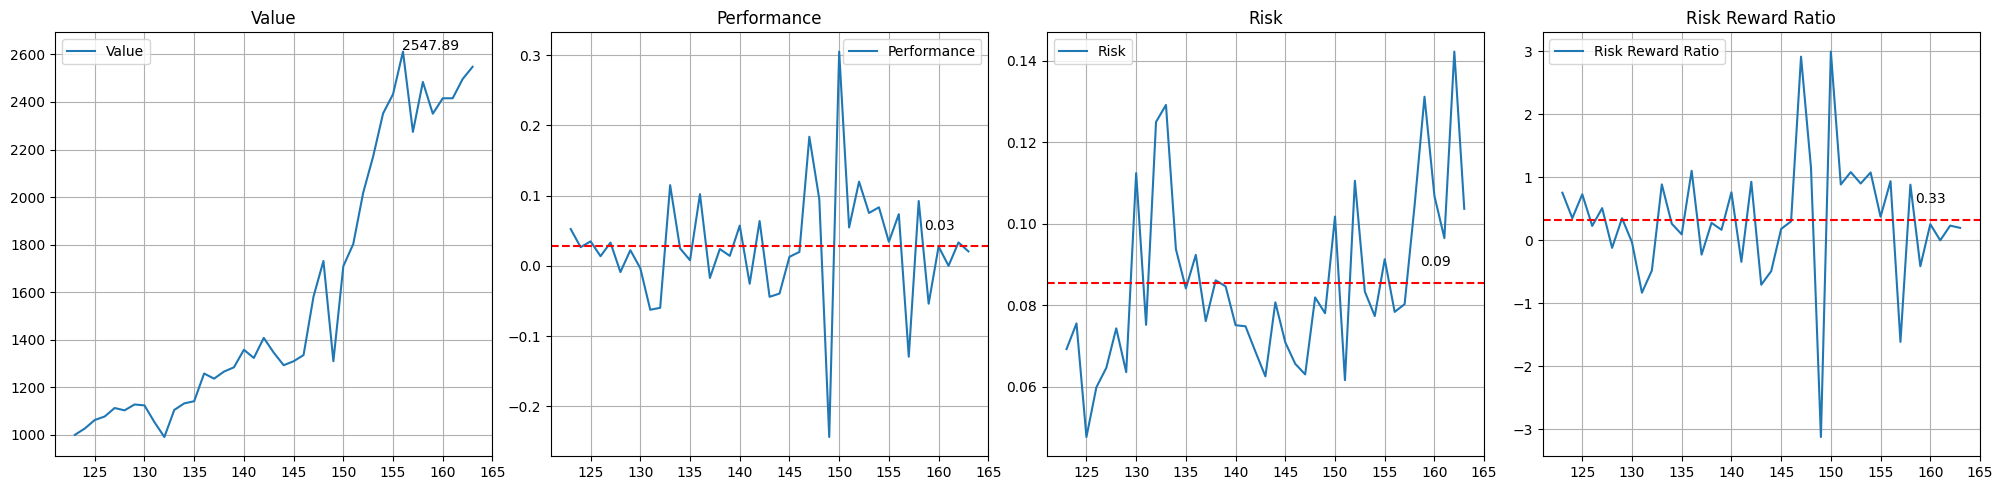
\includegraphics[width=1\textwidth]{best_experts_risk.png}
    \caption{Best Experts Strategy Risk: Fund 3}
    \label{fig:best_experts_risk}
\end{figure}
\begin{figure}[H]
    \centering
    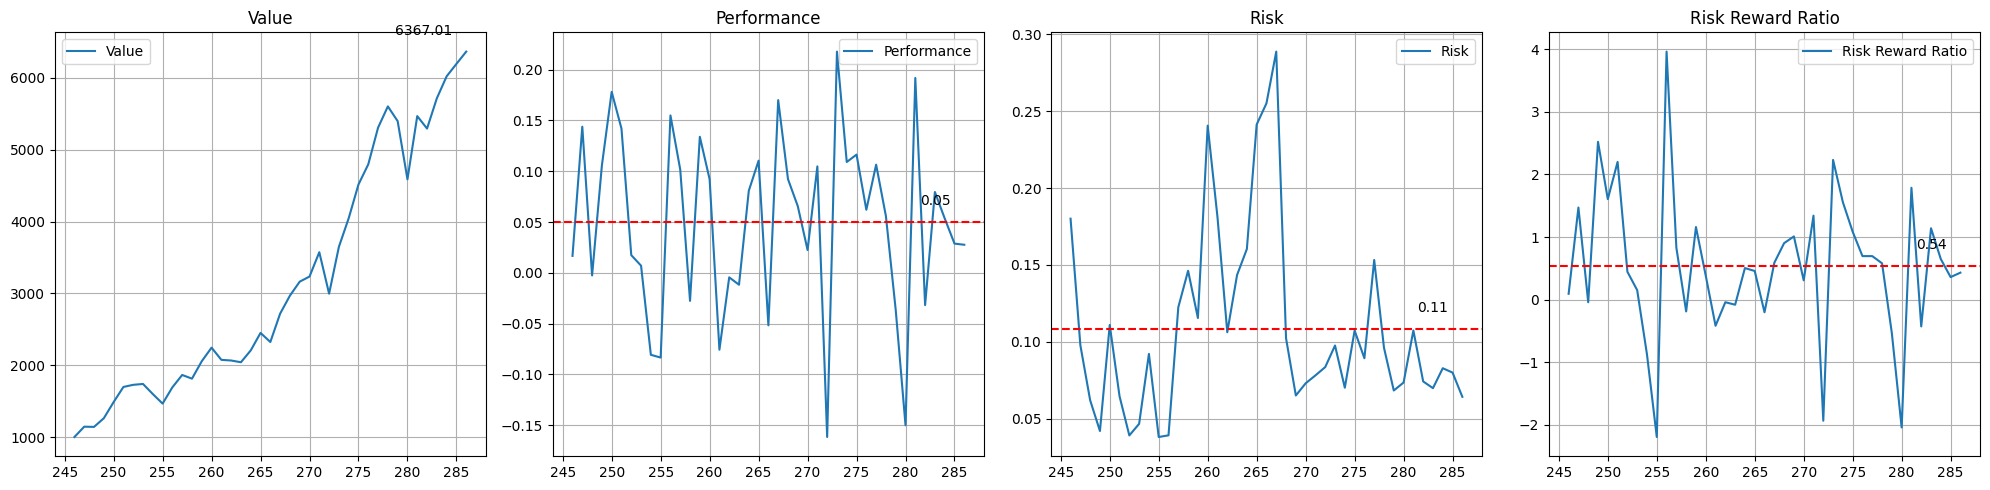
\includegraphics[width=1\textwidth]{best_experts_risk_reward.png}
    \caption{Best Experts Strategy Risk-Reward: Fund 6}
    \label{fig:best_experts_risk_reward}
\end{figure}
%\table to show the best expert values for each of the conditions
\begin{table}[H]
    \centering
    \begin{tabular}{l m{2cm} m{2cm} m{2cm}}
        \toprule
        {Condition} & {Performance} & {Risk} & {Risk-Reward} \\
        \midrule
        Fund No. & 2 & 3 & 6 \\
        Final Value & \$6968.09 & \$2547.89 & \$6367.01\\
        Mean Return & 6.13\% & 2.68\% & 5.05\%\\
        Mean Risk & 18.47\% & 8.55\% & 10.85\%\\
        Mean Risk-Reward & 0.33 & 0.32 & 0.47\\
        \bottomrule
    \end{tabular}
    \caption{Best Experts Strategy Performance}
\end{table}

\subsection{Weighted Majority Algorithm}
\label{subsec:weighted-majority}
We apply the Weighted Majority Algorithm outlined in the methodology section, and optimize $\beta$ for each of the conditions. We get the following results:
\begin{figure}[H]
    \centering
    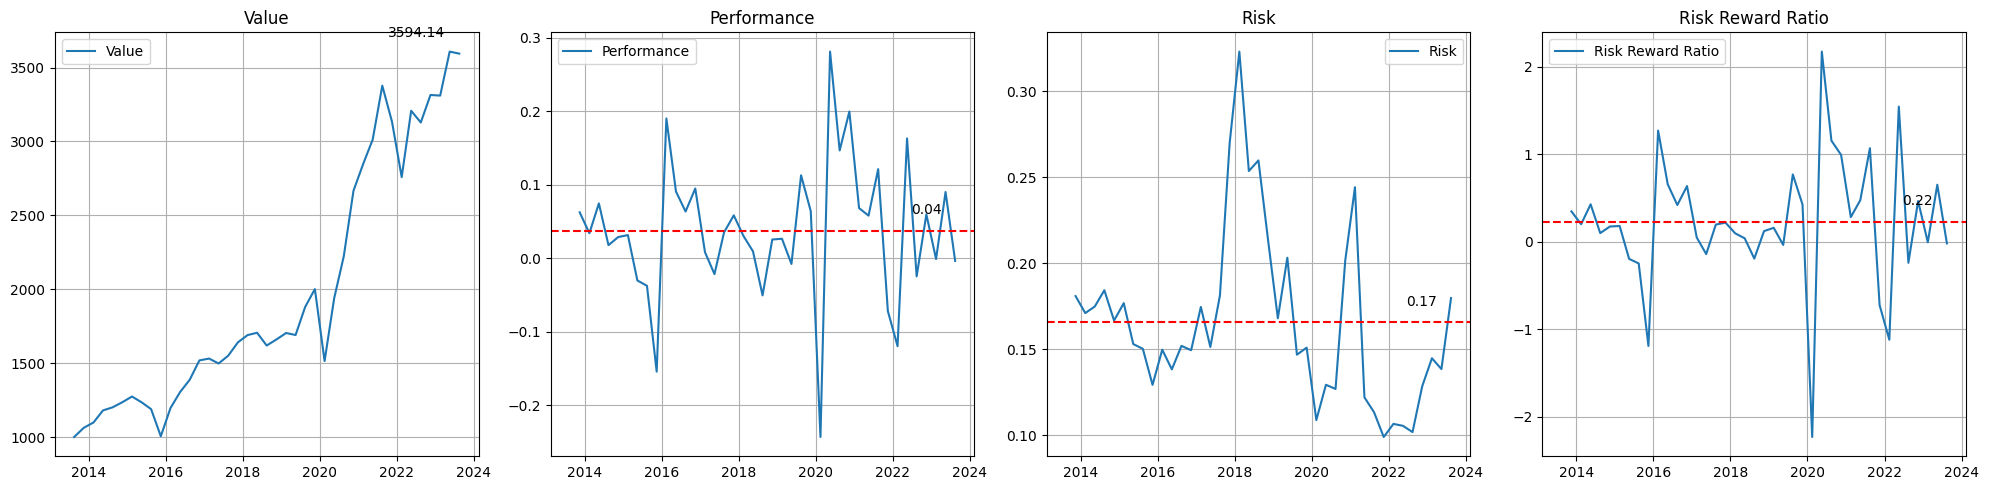
\includegraphics[width=1\textwidth]{weighted_majority.png}
    \caption{Weighted Majority Algorithm Performance}
    \label{fig:weighted_majority}
\end{figure}
\begin{figure}[H]
    \centering
    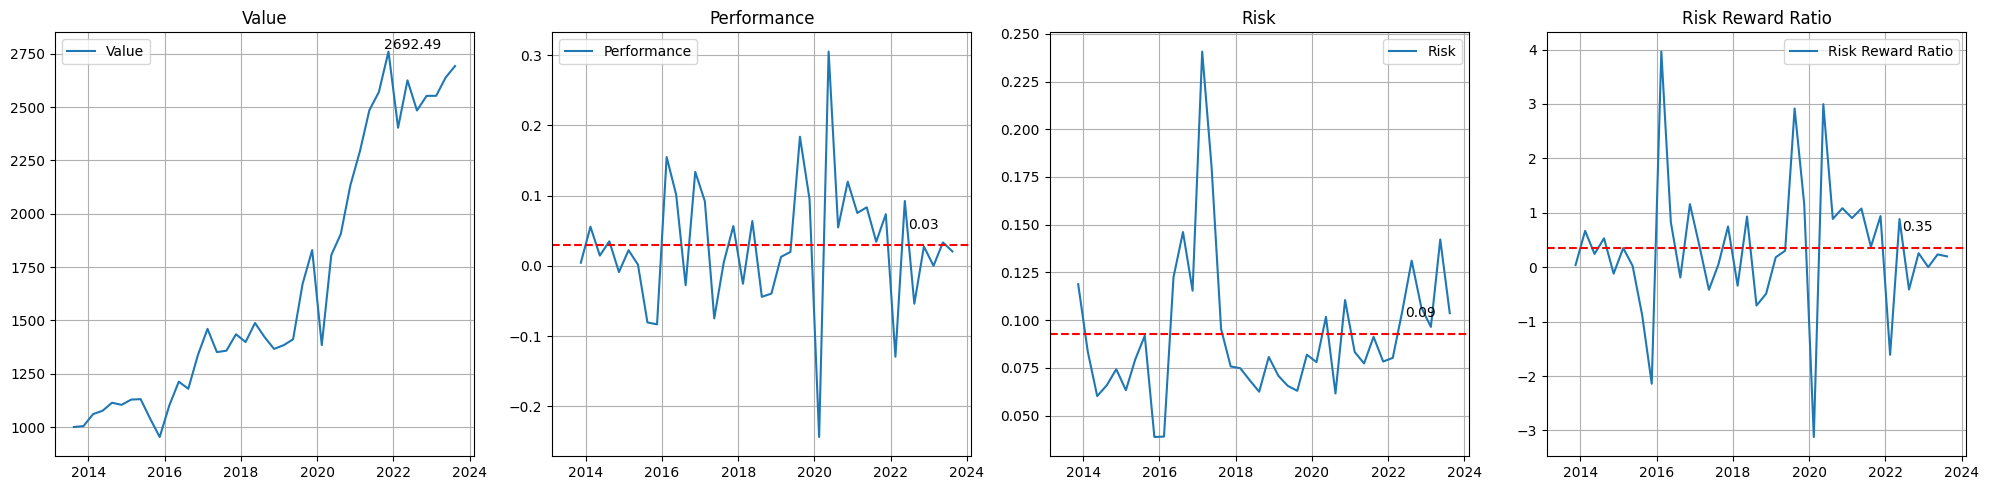
\includegraphics[width=1\textwidth]{weighted_majority_risk.png}
    \caption{Weighted Majority Algorithm Risk}
    \label{fig:weighted_majority_risk}
\end{figure}
\begin{figure}[H]
    \centering
    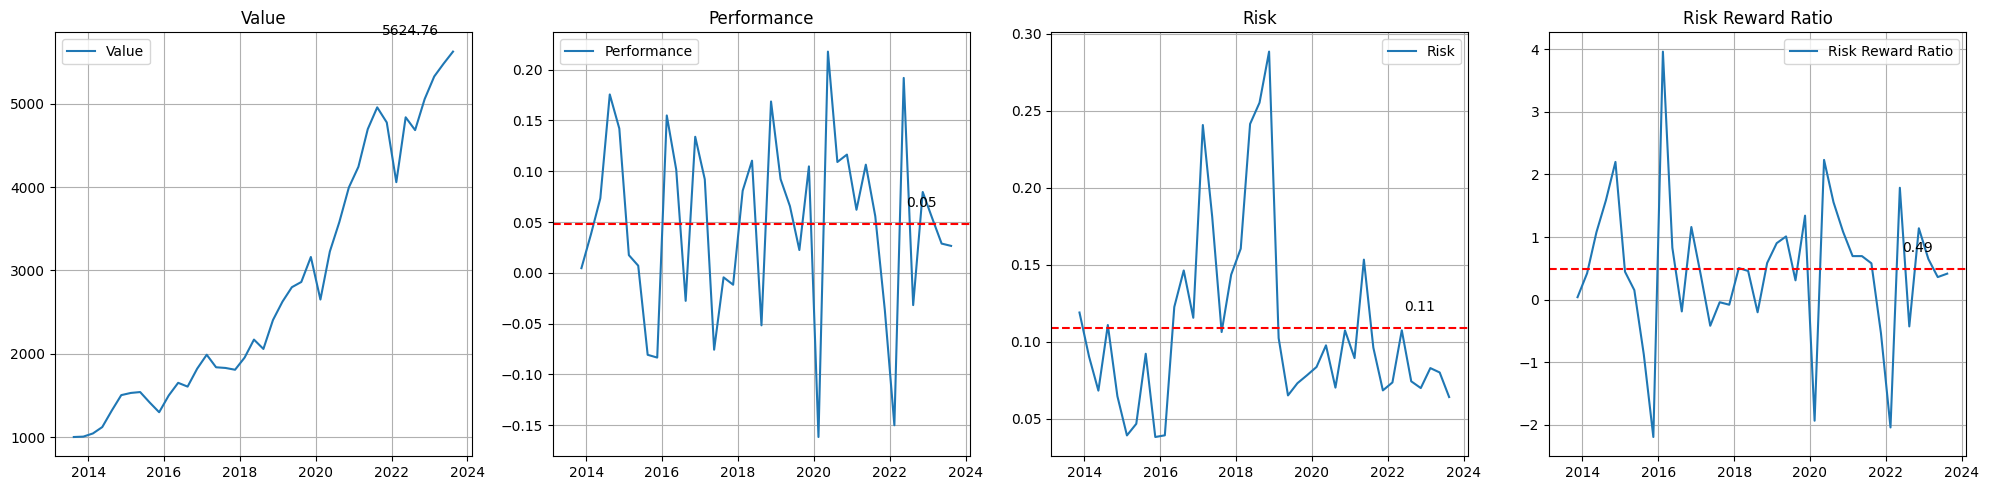
\includegraphics[width=1\textwidth]{weighted_majority_risk_reward.png}
    \caption{Weighted Majority Algorithm Risk-Reward}
    \label{fig:weighted_majority_risk_reward}
\end{figure}
%\table to show the best expert values for each of the conditions
\begin{table}[H]
    \centering
    \begin{tabular}{l m{2cm} m{2cm} m{2cm}}
        \toprule
        {Condition} & {Performance} & {Risk} & {Risk-Reward} \\
        \midrule
        Optimal Beta & 0.82 & 0.01 & 0.01\\
        Final Value & \$3594.14 & \$2692.49 & \$5624.76\\
        Mean Return & 3.69\% & 2.91\% & 4.79\%\\
        Mean Risk & 16.56\% & 9.27\% & 10.86\%\\
        Mean Risk-Reward & 0.22 & 0.31 & 0.44\\
        \bottomrule
    \end{tabular}
    \caption{Weighted Majority Algorithm Performance}
\end{table}
We see that the Weighted Majority Algorithm is unable to outperform but is able to get close to the best expert in terms of risk and risk-return ratio by optimizing $\beta$.

    \begin{figure}[H]
    \centering
    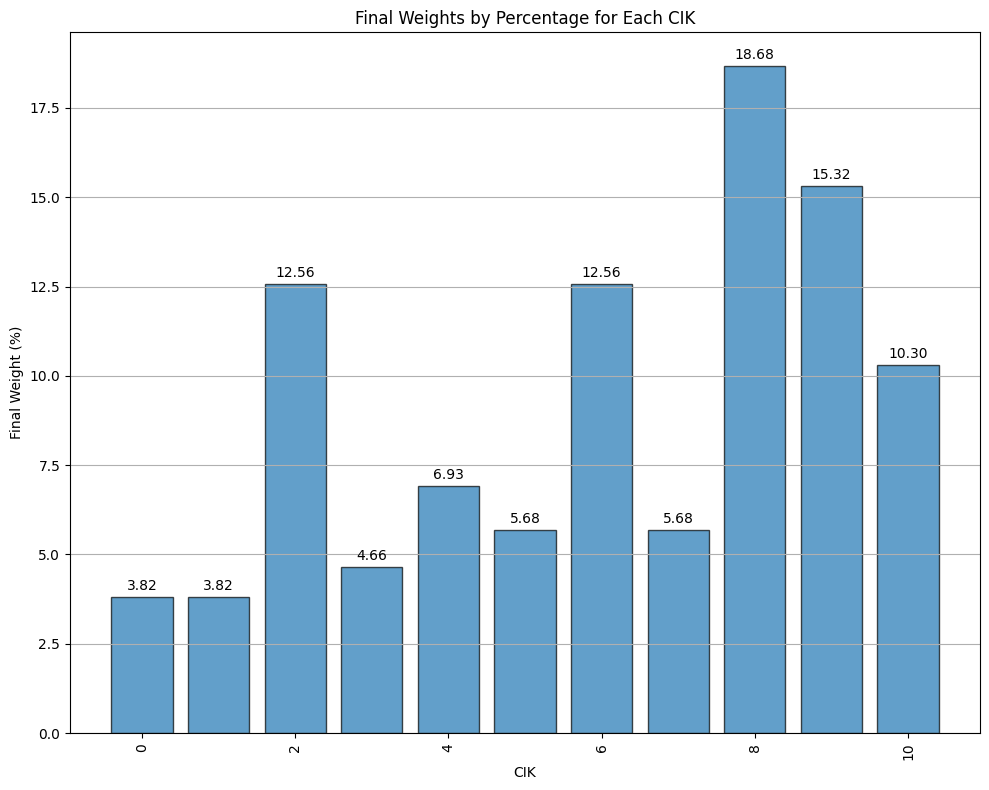
\includegraphics[width=0.8\textwidth]{weighted_majority_final_weights.png}
    \caption{Weighted Majority Algorithm Performance Weights}
        \label{fig:weighted_majority_final_weights}
    \end{figure}

    \begin{figure}[H]
        \centering
        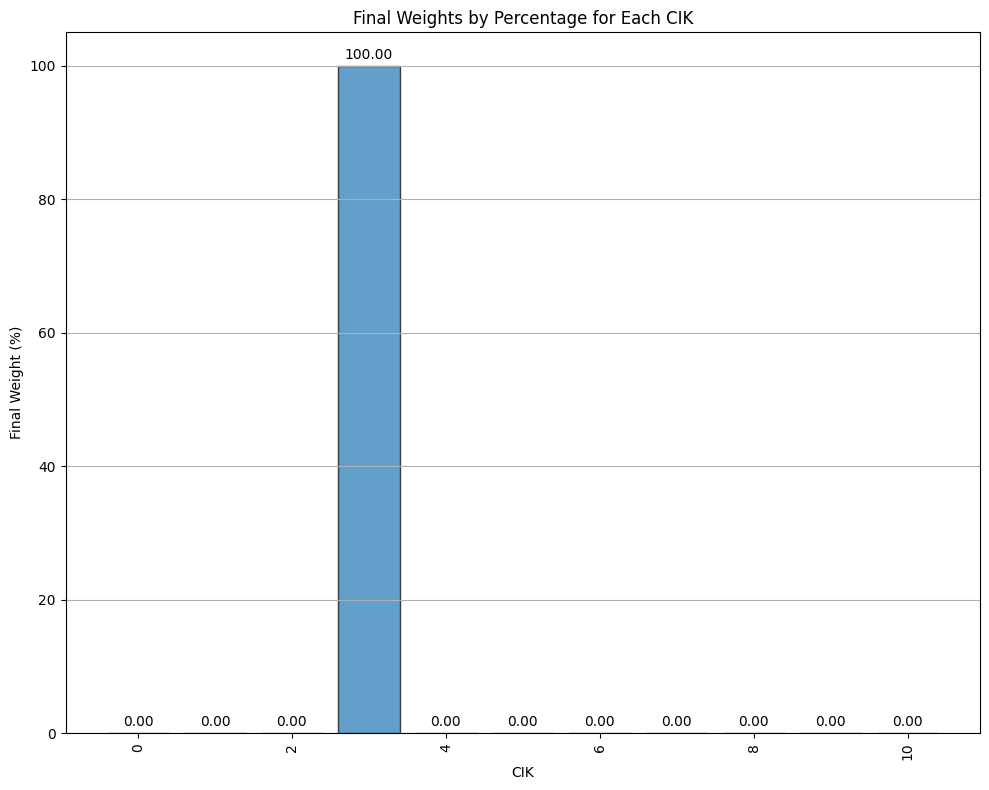
\includegraphics[width=0.8\textwidth]{weighted_majority_risk_final_weights.png}
        \caption{Weighted Majority Algorithm Risk Weights}
        \label{fig:weighted_majority_risk_final_weights}
    \end{figure}

    \begin{figure}[H]
        \centering
        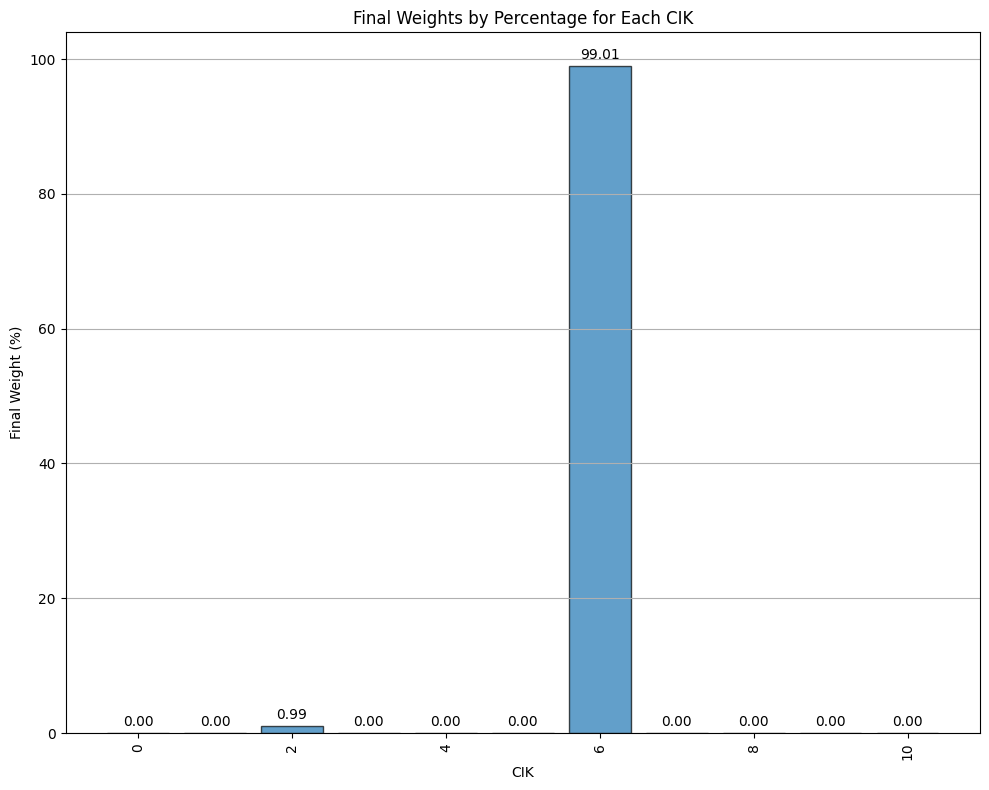
\includegraphics[width=0.8\textwidth]{weighted_majority_risk_reward_final_weights.png}
        \caption{Weighted Majority Algorithm Risk-Reward Weights}
        \label{fig:weighted_majority_risk_reward_final_weights}
    \end{figure}

In fact, looking at the last two, we see that the reason the optimal beta values for Risk and Risk-Reward is so low is because it takes the opportunity to invest in the best expert as much as possible, and then never changes the weights. This means that the Weighted Majority Algorithm works to reduce the number of mistakes made specifically for the cases of Risk and Risk-Reward. 

\subsection{Random Weighted Majority Algorithm}
\label{subsec:random-weighted-majority}
How about the Random Weighted Majority Algorithm? We apply the Random Weighted Majority Algorithm outlined in the methodology section, and instead of using a optimized $\beta$, we use $\beta=\{0.125, 0.25, 0.5\}$ for performance. We get the following results simulating the Random Weighted Majority Algorithm:
\begin{figure}[H]
    \centering
    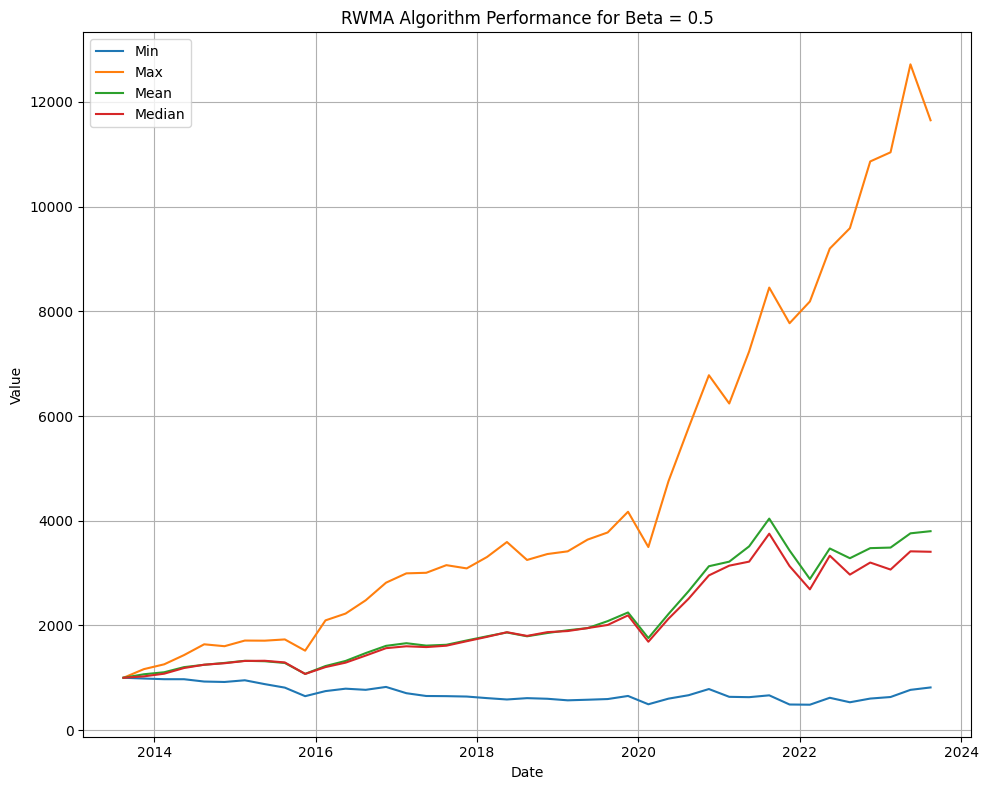
\includegraphics[width=1\textwidth]{rwma_0.5.png}
    \caption{Random Weighted Majority Algorithm Performance: $\beta=0.5$}
    \label{fig:rwma_0.5}
\end{figure}
\begin{figure}[H]
    \centering
    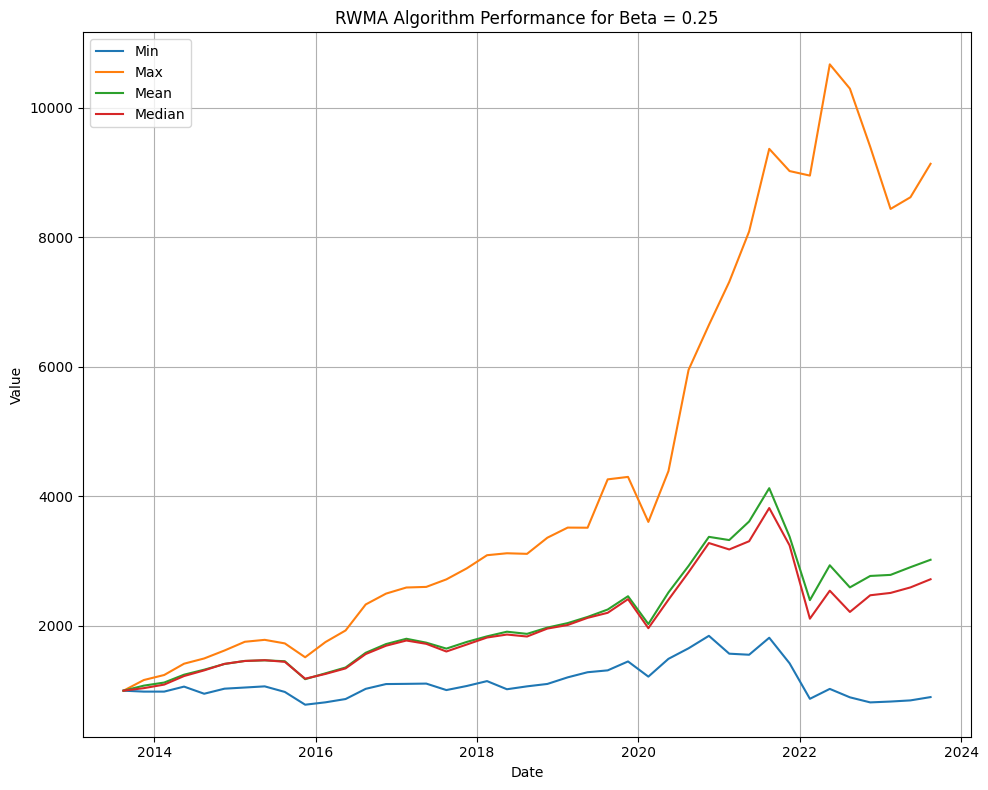
\includegraphics[width=1\textwidth]{rwma_0.25.png}
    \caption{Random Weighted Majority Algorithm Performance: $\beta=0.25$}
    \label{fig:rwma_0.25}
\end{figure}
\begin{figure}[H]
    \centering
    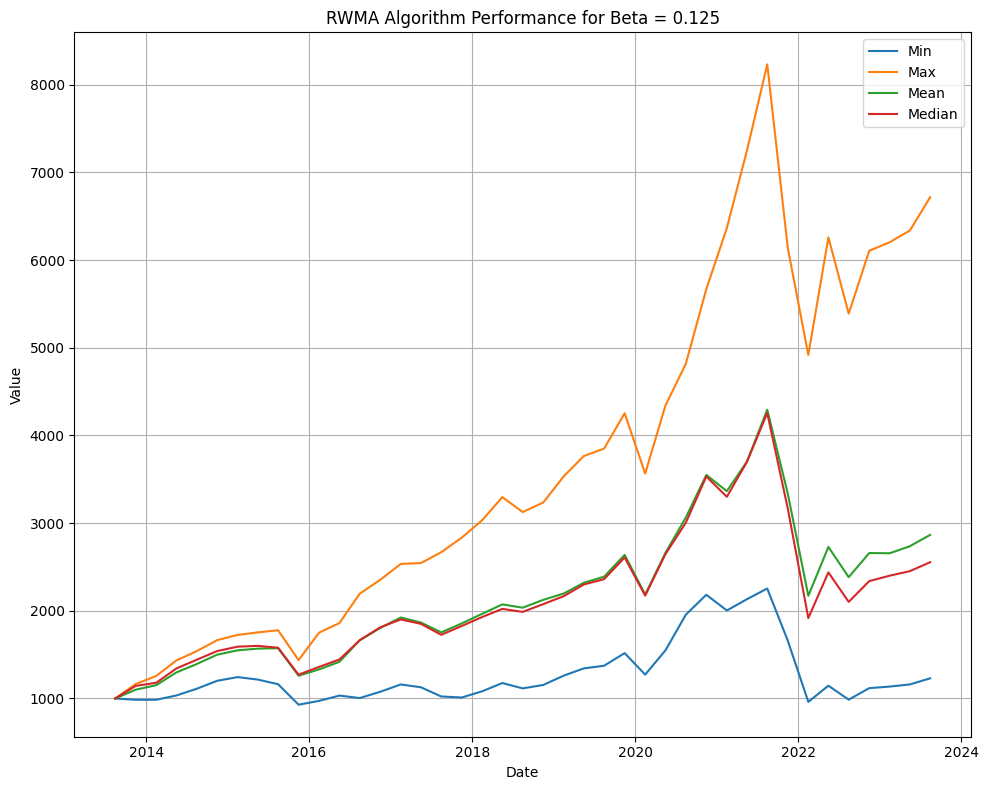
\includegraphics[width=1\textwidth]{rwma_0.125.png}
    \caption{Random Weighted Majority Algorithm Performance: $\beta=0.125$}
    \label{fig:rwma_0.125}
\end{figure}
This seems to show what we have learnt, which is that as we reduce our $\beta$, we are able to reduce the number of mistakes made and get closer to the best expert.

\subsection{Modified Greedy Algorithm}
Lastly, we apply the Modified Greedy Algorithm outlined in the methodology section, and see if we can get to our best expert without having to apply weights or randomization. Specifically, we know that the weights of our modified greedy algorithm will be the same as the weights in WMA for each timestep $t$, assuming we are looking at the same $\beta$ value, but we select the best expert at each time $t$ to invest in by looking at who has the highest weight at time $t-1$ instead of weighing the experts. 

What we want to do here is to fix $\beta$ like we would in a real-world scenario, and see if which strategy gives the best performance. Beyond just getting to the best expert, which model actually gives better returns when, in this case, we keep $\beta=0.125$?
\begin{figure}[H]
    \centering
    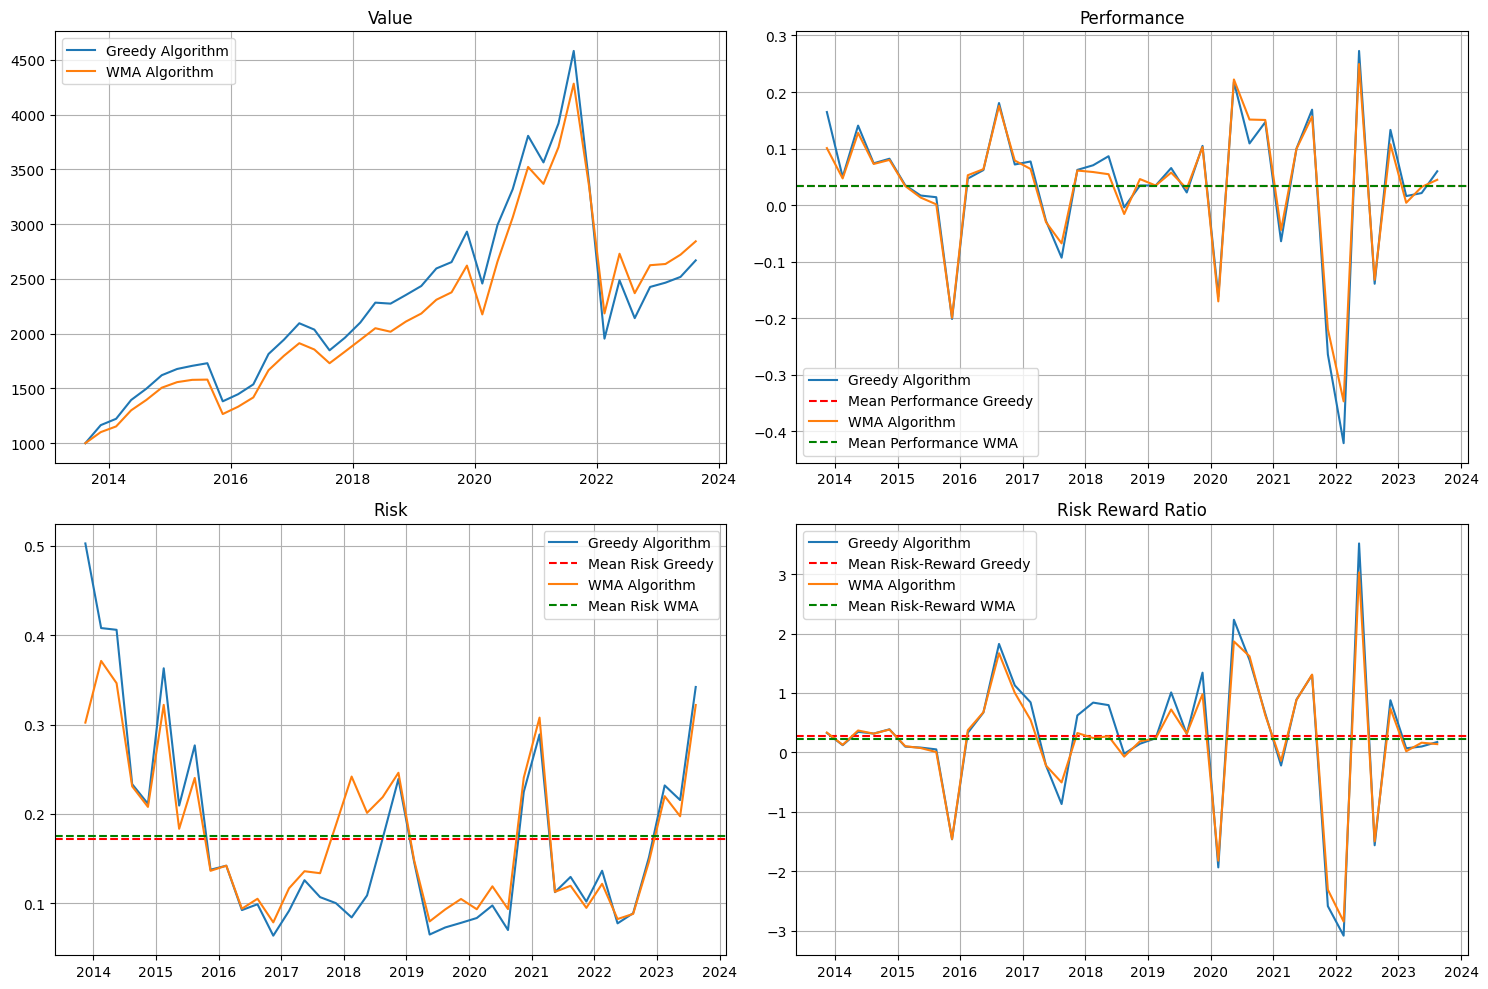
\includegraphics[width=0.8\textwidth]{performance_comparison.png}
    \caption{Performance Comparison}
    \label{fig:performance_comparison}
\end{figure}
\begin{figure}[H]
    \centering
    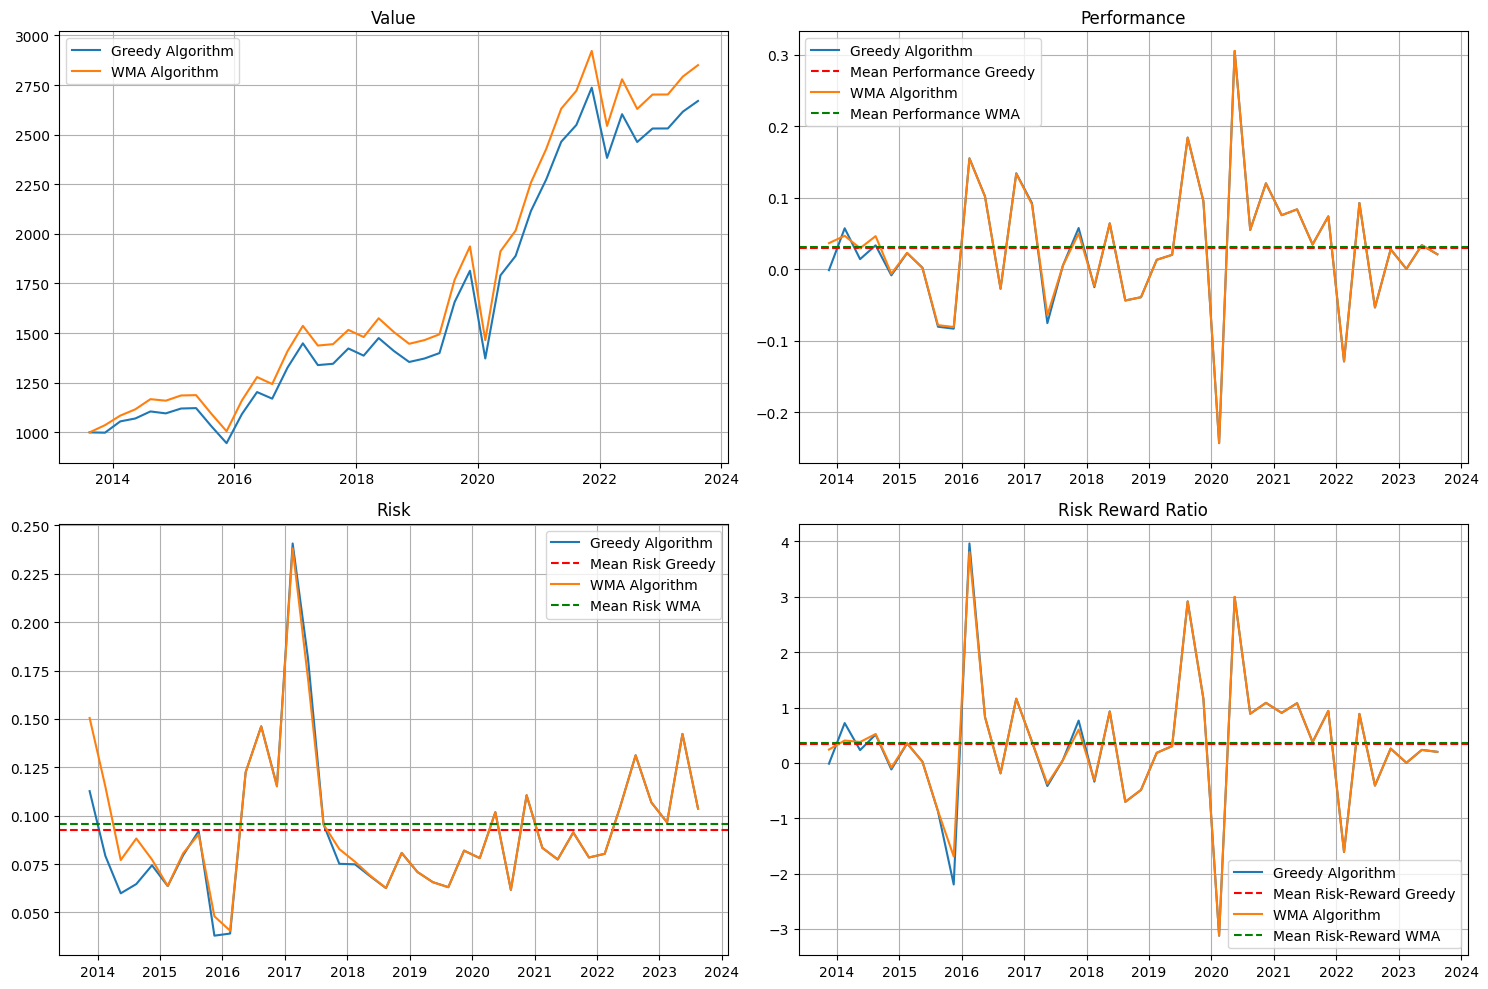
\includegraphics[width=0.8\textwidth]{risk_comparison.png}
    \caption{Risk Comparison}
    \label{fig:risk_comparison}
\end{figure}
\begin{figure}[H]
    \centering
    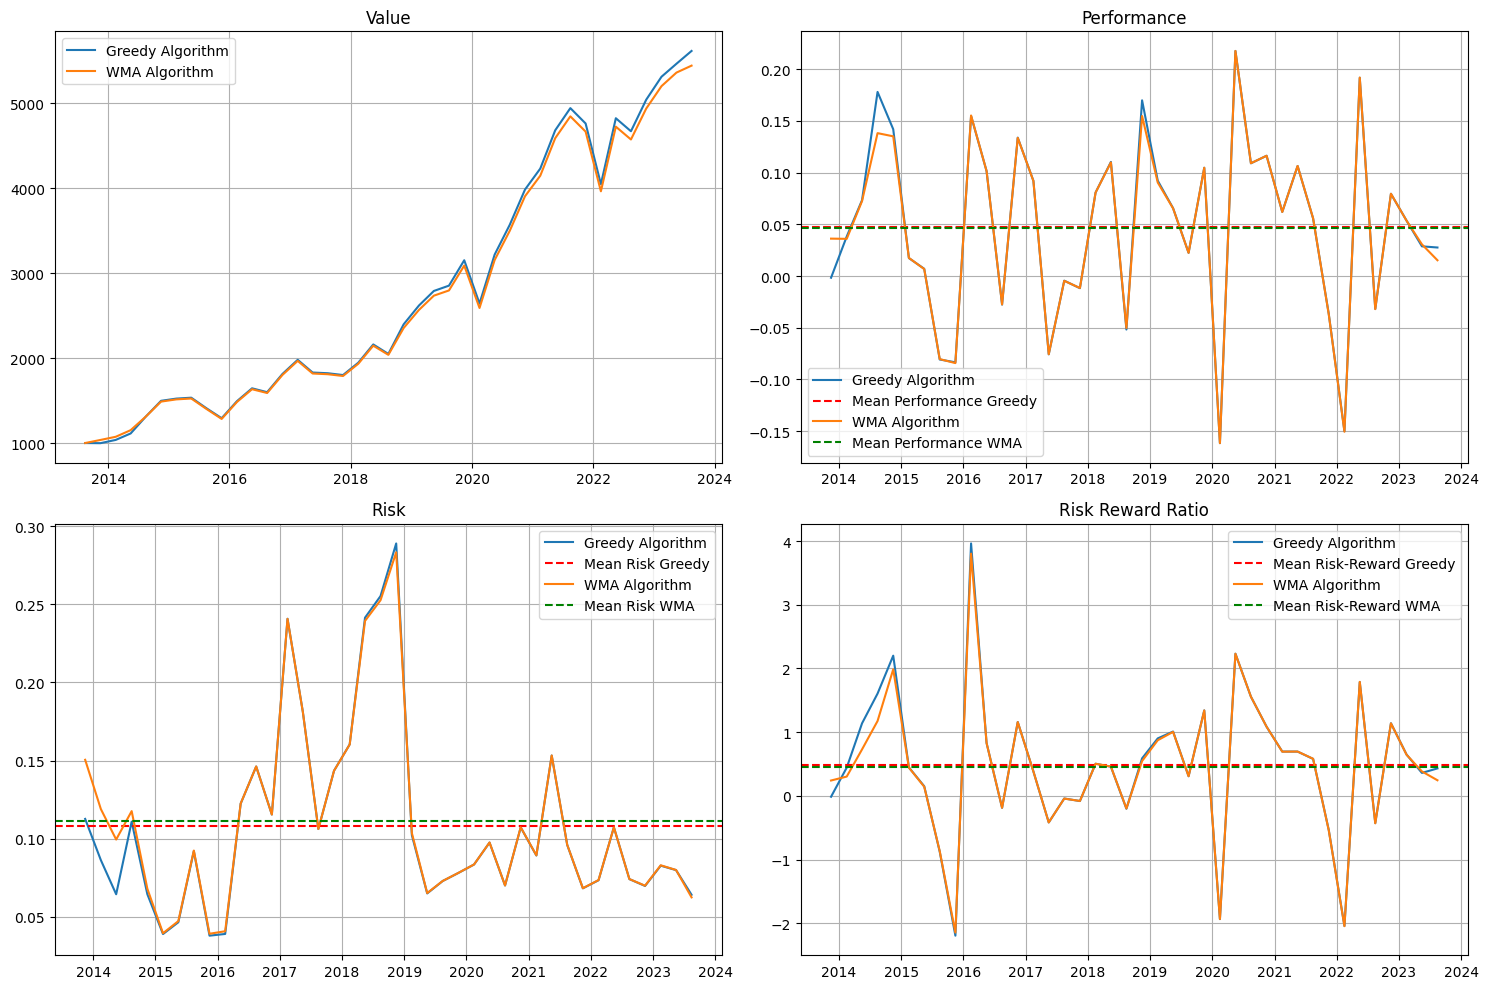
\includegraphics[width=0.8\textwidth]{risk_reward_comparison.png}
    \caption{Risk-Reward Comparison}
    \label{fig:risk_reward_comparison}
\end{figure}

We see that the Modified Greedy Algorithm is unable to outperform WMA in terms of performance, but is able to get closer to best expert in terms of risk and risk-reward ratio

\section{Conclusion}
\label{sec:conclusion}
In this paper, we compared various strategies for combining expert advice, particularly in the context of stock market prediction using 13F filings from top hedge funds. We analyzed the performance, risk, and risk-reward ratios of different algorithms: Equal Weighted Strategy, Best Experts Strategy, Weighted Majority Algorithm (WMA), Random Weighted Majority Algorithm (RWMA), and Modified Greedy Algorithm.

The standout observation was the performance of the Modified Greedy Algorithm. Although it did not achieve the highest returns in terms of raw performance, it excelled in minimizing risk and optimizing the risk-reward ratio. This superior performance in risk and risk-reward is likely due to its approach of going all-in on the best expert faster than WMA. By quickly committing to the top-performing expert based on current weights, the Modified Greedy Algorithm effectively reduces exposure to underperforming experts, thereby enhancing overall portfolio stability and risk-adjusted returns.

In conclusion, the choice of algorithm depends on the specific goals and risk tolerance of the investor. For those seeking balanced performance with moderate risk, WMA and RWMA are suitable options. However, for investors prioritizing risk management and optimal risk-reward ratios, the Modified Greedy Algorithm presents a compelling strategy.

\end{document}